\documentclass[PICOReport.tex]{subfiles}

\begin{document}

{\bf Gravitational waves and inflation} \\[0.3cm] 
Measurements of the CMB together with Einstein's theory of general relativity imply that the observed density perturbations must have been created long before the CMB was released, and rather remarkably even before the universe became filled with a hot and dense plasma of fundamental particles. What generated these perturbations is one of the biggest questions in cosmology.

While the dynamics of the plasma produces some amount of gravitational waves, the amplitude is too small to be detected in existing or planned CMB experiments. So any imprint of gravitational waves on the cosmic microwave background detected by PICO would constitute evidence for gravitational waves from the same primordial period that created the density perturbations. Because the dynamics of gravitational waves is essentially unaffected by the plasma physics, they would be a pristine relic left over from the earliest moments of our universe, and their properties would shed light on the mechanism that created the primordial perturbations that grew into the anisotropies of the CMB and the stars and galaxies around us. Knowledge of the strength of the signal and their statistical properties would transform our understanding of many areas of fundamental physics. 


Inflation, a period of nearly exponential expansion of the early universe, is the leading paradigm explaining the origin of the primordial density perturbations. It predicts a nearly scale invariant spectrum of primordial gravitational waves originating from quantum fluctuations. Thus, a detection of these gravitational waves would be the first detection of phenomenon associated with quantum gravity. Because the spectrum is scale-invariant, one may hope to detect primordial gravitational waves over a wide range of frequencies including, for example, at LIGO or LISA frequencies. However, as a consequence of the expansion of the universe, the energy density in the gravitational waves rapidly dilutes with increasing frequency, and observations of the CMB provide the easiest, and for the foreseeable future only way to detect these gravitational waves. 


\begin{figure}[!htb]
\centering
\hspace{-0.15in}
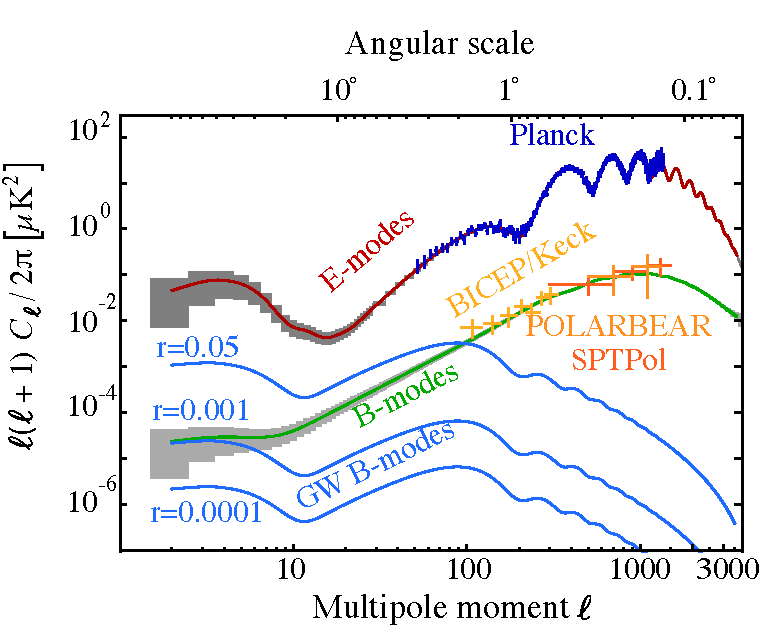
\includegraphics[width=3in]{images/cmb_powspec_PICOv2.pdf}
\hspace{-0.15in}
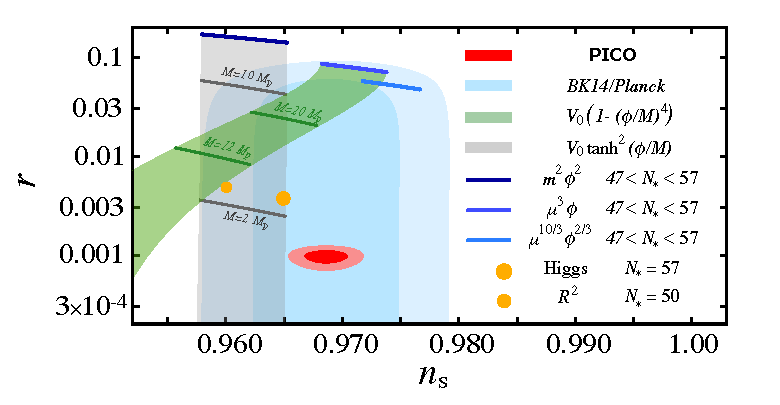
\includegraphics[width=3.6in]{images/nsrlabeledrp001_PICOv1.pdf}
\caption{power spectrum place holder}
\label{fig:clbb}
\end{figure}

The strength of the signal, often quantified by the tensor-to-scalar ratio $r$, is a direct measure of the expansion rate of the universe during inflation. Together with the Friedmann equation, this reveals one of the most important characteristics of inflation, its energy scale. PICO will be able to detect primordial gravitational waves if inflation occurred at an energy scale of at least $4\times 10^{15}\,\rm{GeV}$. A detection would have profound implications for fundamental physics because it would provide evidence for a new energy scale, and would allow us to probe physics at energies far beyond the reach of terrestrial colliders.

The signal would have two contributions, one on degree angular scales or multipoles of $\ell\sim 80$, typically referred to as the recombination peak, and another contribution for multipoles of $\ell\lesssim 20$ from reionization. The contribution from reionization is expected to be strongest relative to the contribution from weak lensing and instrumental noise. No sub-orbital experiment has meaningfully measured modes at $\ell<40$ and a satellite like PICO is the most suitable approach to reach the lowest multipoles.  

There are two classes of slow-roll inflation that naturally explain the observed value of the spectral index of primordial fluctuations, $n_s$. The first class is characterized by potentials of the form $V(\phi)\propto\phi^p$. This class includes many of of the simplest models of inflation, some of which have already been strongly disfavored by existing observations. If the constraints on the spectral index tighten by about a factor 2 with the central value unchanged, and the upper limits on $r$ improve by an order of magnitude, this class would be ruled out. 

%\begin{figure}[!htb]
%\centering
%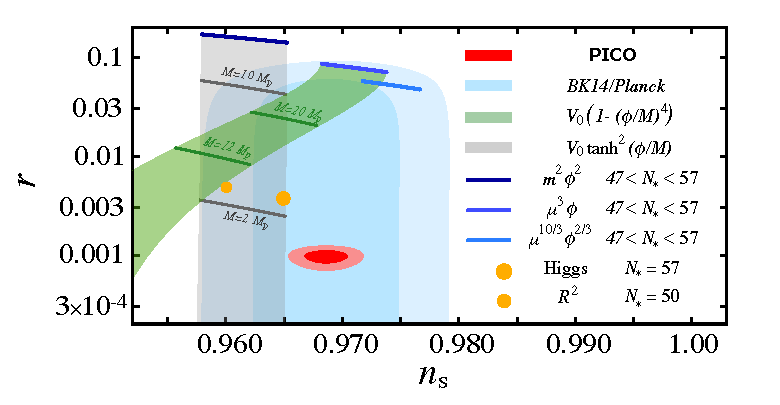
\includegraphics[width=5in]{images/nsrlabeledrp001_PICOv1.pdf}
%\caption{nsr placeholder}
%\label{fig:nsr}
%\end{figure}

The second class is characterized by potentials that exponentially approach a plateau and include $R^2$ inflation. This model predicts a tensor-to-scalar ratio of $r\sim 0.003$. All models in this class with a characteristic scale in the potential that is larger than the Planck scale predict a tensor-to-scalar ratio
of $r\gtrsim 0.001$, and an experiment like CMB-S4 could exclude these scenarios. However, there are models such as the Goncharov-Linde model with a somewhat smaller characteristic scale that predict a tensor-to-scalar ratio of $r\sim 4\times 10^{-4}$. 



In the absence of a detection, PICO would limit the amount of gravitational waves to $r<10^{-4}$ at $95\%$ CL. This is stronger than current upper limits by three orders of magnitude, and stronger than those expected for the ground-based experiment CMB-S4 by an order of magnitude. 


Models of inflation, or the early universe more generally, differ in their predictions for the scalar spectral index $n_{\rm s}$ and its scale dependence, often referred to as the running of the spectral index $n_{\rm run}$. With its high resolution and low noise levels, PICO will improve the constraints on $n_{\rm s}$ and $n_{\rm run}$ by a factor of about two. In addition, PICO will probe the statistical properties of the primordial fluctuations over a wide range of scales with exquisite precision and improve constraints on departures from Gaussianity by a factor $2-3$.\\

{\bf Light relics}\\[0.3cm]
In the inflationary paradigm, the universe was reheated to temperatures of at least 10 MeV and perhaps as high as $10^{12}$ GeV.  
At these high temperatures, even very weakly interacting or very massive particles, such as those arising 
in extensions of the standard model of particle physics, can be produced in large abundances~\cite{1979ARNPS..29..313S,Bolz:2000fu}.  As the universe expands and cools, 
the particles fall out of equilibrium, leaving observable signatures in the CMB power spectra. 
Through these effects the CMB is a sensitive probe of neutrino and of other particles' properties.  

One particularly compelling target is the effective number of light relic particle species $\Neff$, also called the effective 
number of neutrinos. The canonical value with three neutrino families is $\Neff = 3.046$. Additional light particles 
%in thermal equilibrium with the Standard model particles at any point in our history, it will 
contribute a change to $\Neff$ of $\Delta \Neff \geq 0.027\,g$ where $g \geq 1$ is the number of 
degrees of freedom of the new particle~\cite{Brust:2013xpv,Baumann:2016wac}.  
This defines a target of $\sigma(\Neff) < 0.027$ for future CMB observations. 
Either a limit or detection of $\Delta \Neff$ at this level would provide powerful insights into the basic constituents 
of matter. 

Forecasts for $\Neff$ are shown in Figure~\ref{fig:Neff_future}.  The two most important parameters for improving constraints
are the fraction of sky observed $f_{\rm sky}$ and the noise. Achieving both larger $f_{\rm sky}$ and
lower noise are strengths of PICO compared to other platforms. 
Our baseline mission nearly reaches the target constraint with $g=1$. 
A newly designed mission with only 10 times higher sensitivity will reach $\sigma(\Neff) < 0.025$.  A high precision measurement of the 
CMB in temperature and polarization is the only proven approach to reach this important threshold.  

\begin{figure}[t!]
\begin{center}
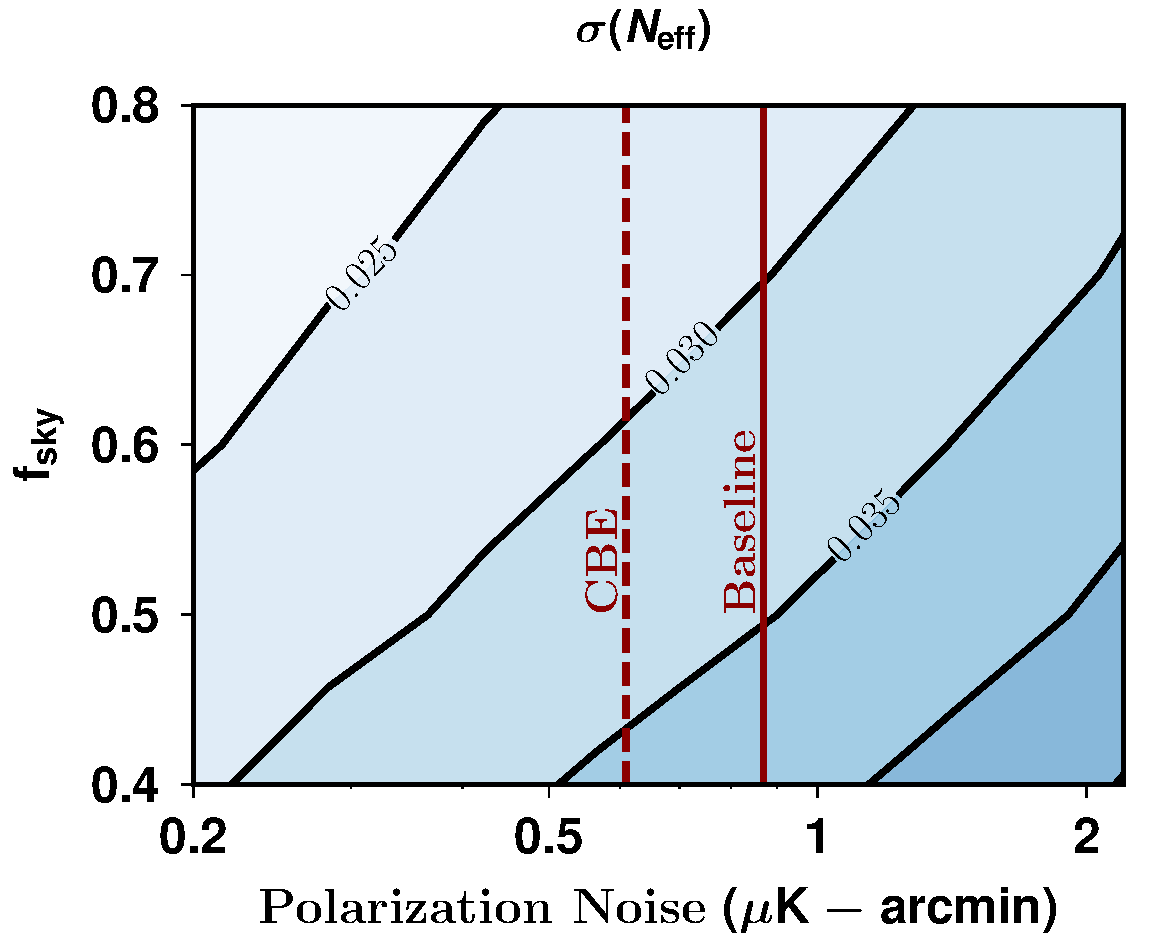
\includegraphics[width=0.45\textwidth]{images/Neff_final.pdf}
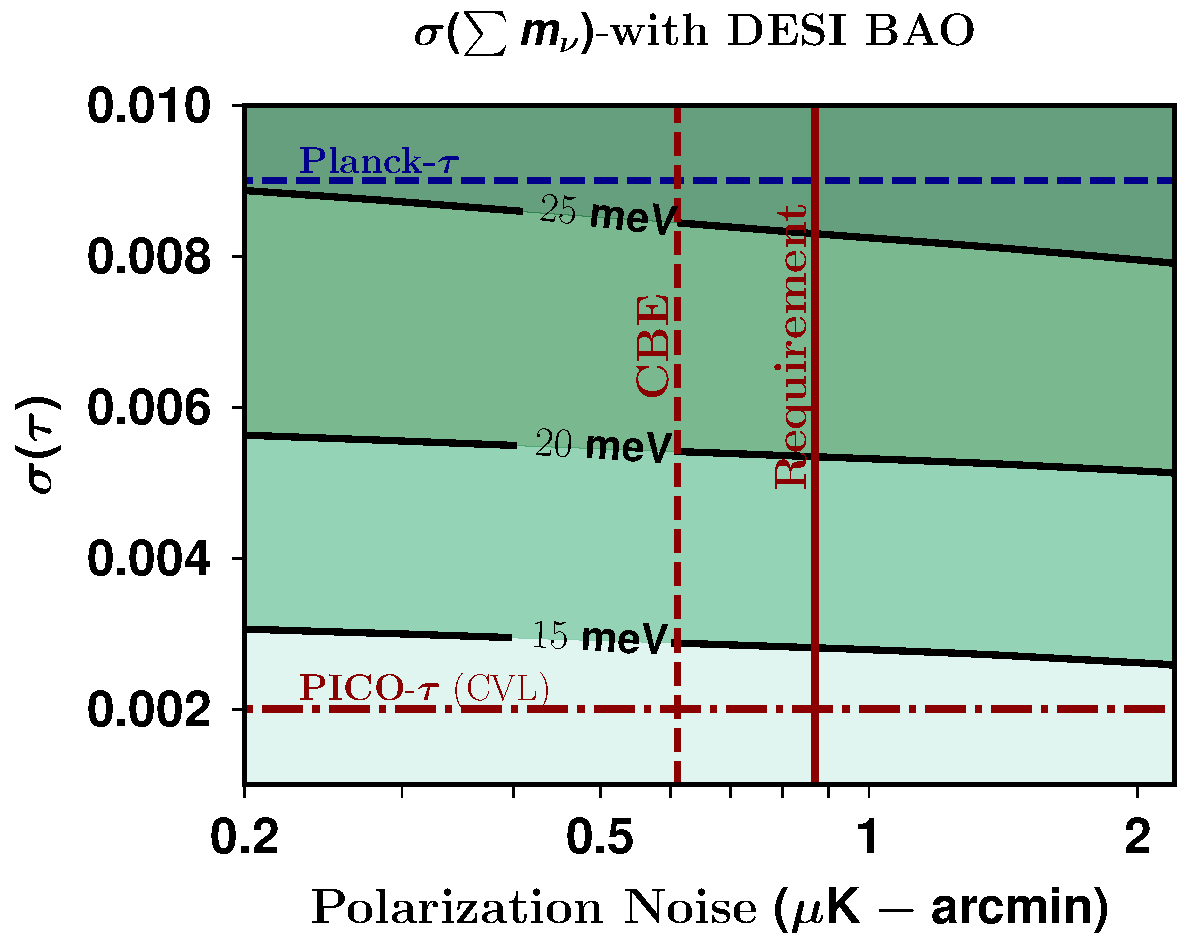
\includegraphics[width=0.47\textwidth]{images/Mnu_tauprior_final.pdf}
\vspace{-0.15in}
\caption{ \small \setlength{\baselineskip}{0.95\baselineskip}
$\Neff$ uncertainty as a function of noise and sky fraction (left) and sum of 
neutrino masses uncertainty as a function of noise and the uncertainty in the measurement of $\tau$, 
for 0.7 sky fraction (right). The resolution assumed is 5'.  
Vertical lines denote the expected performance of the baseline mission. 
The upper blue dashed line is the current \planck~limit; the lower grey dashed line is the limit from cosmic variance 
limited measurement of $\tau$. All forecasts assume internal delensing of the $T$ and $E$-maps~\cite{Green:2016cjr}, 
including residual non-Gaussian covariances.  The $\sum m_\nu$ forecasts include DESI BAO.  
\label{fig:Neff_future} }
\end{center}
\vspace{-0.15in}
\end{figure}

Many light relics of the early universe are not stable. They decay, 
leaving faint evidence of their past existence on other tracers. The relics with sufficiently long lifetime to survive few minutes, 
past the epoch of light element synthesis, leave a signature on the helium fraction $Y_p$.  If they decay 
by the time of recombination, their existence through this period is best measured through the ratio of $\Neff$ to $Y_p$. 
PICO's cosmic variance limited determination 
of the $E$ mode power spectra will improve current limits for these quantities by
a factor of five thus eliminating sub-MeV mass thermal relics. 
%Spectrum distortion measurements give additional constraints on the lifetime and abundance 
%of such relics \citep{Sarkar1984, Kawasaki1986, Hu1993b, Chluba2011therm}. 

Cosmological measurements have already confirmed the existence of one relic that lies beyond the 
Standard Model: dark matter. For a conventional WIMP candidate, the CMB places very stringent 
constraints on its properties through the signature of its annihilation on the $T$ and $E$ 
spectra \citep{Peebles2000, Chen2004, Padmanabhan2005}.  \planck\ currently excludes WIMPs with mass 
$m_{\rm dm}< 16$ GeV and a future CMB mission could reach $m_{\rm dm} < 45$ GeV for $f_{\rm sky} =0.8$.  The 
CMB provides the most stringent constraints on the dark matter annihilation cross section for dark matter 
in this mass range.  
%The CMB is complimentary to direct detection experiments which probe the scattering 
%cross-section of dark matter with standard model particles.

%A dark matter candidate can also have a slow decay to Standard models particles which is 
%similarly constrained by the CMB~\cite{Chen2004, Zhang2007, Diamanti2014, Slatyer:2016qyl}.  Current and future CMB limits on the lifetime of $\tau \gtrsim 10^{25}$ s are somewhat weaker than indirect detection limits of $\tau > 10^{24-28}$~s~\cite{Essig:2013goa}.  

A particle-independent approach is to constrain dark matter interactions that would 
affect the evolution of the effective dark matter fluid and its interactions with baryons or photons.  The simplest example is 
to constrain the baryon-dark matter cross section through its effective coupling of the two fluids~\cite{Dvorkin:2013cea}.  
These couplings affect the evolution of fluctuations and ultimately the $T$ and $E$ spectra. The current limits of $\sigma \lesssim 10^{-31}-10^{-34}\,{\rm cm}^2 \times (m_{\rm dm} / {\rm MeV})$ can be competitive with direct detection for sub-GeV masses.  
More exotic dark sectors that include long-range forces can produce an even richer phenomenology in the CMB and in the large-scale structure 
without necessarily producing an associated signature in direct detection experiments or 
indirect searches (e.g.~\cite{Cyr-Racine:2013fsa,Buen-Abad:2015ova,Lesgourgues:2015wza}). 

%Interactions of dark matter with standard model particles can also be constrained through 
%measurements of spectral distortions \cite{Yacine2015DM}. 
%Chluba et al. showed 
%As the universe expands, the matter cools. Compton interactions with electrons keep the normal matter at the CMB 
%temperature until well after recombination. This leads to a small distortion of the CMB with a negative chemical 
%potential~\citep{Chluba2011therm}. In a similar manner, interactions of DM with electron, protons or directly 
%with CMB photons can lead to a distortion. 
%Current constraints from FIRAS's spectrum measurement are most sensitive to small dark matter
%mass, $m_{\rm X}\lesssim 0.2\,{\rm MeV}$, but these could be extended to $m_{\rm X}\lesssim 1\,{\rm GeV}$ with a 
%Probe-class mission, thus testing DM interaction down to cross-sections 
$\sigma\simeq 10^{-39}-10^{-35}\,{\rm cm}^2$~\cite{Yacine2015DM}. 
%This provides new constraints on the low mass end, $m_{\rm X}\lesssim 10\,{\rm MeV}$ and improves existing limits~\cite{Essig2012PhRvL.109b1301E, Boehm2014MNRAS.445L..31B} by up to a factor of $\simeq 50$. 
%Spectral distortion measurements also open a new avenue for testing dark matter-proton interactions~\cite{Yacine2015DM}.

A host of other physical phenomena including the existence and properties of axions, primordial magnetic fields, and 
superconducting strings, leave signatures on the spectrum of the CMB and can therefore be constrained by 
the sensitive measurements  of a future Probe~\cite[e.g.,][]{Jedamzik2000, Tashiro2012, Dolgov2013, Tashiro2013, Caldwell2013}.\\


{\bf Neutrino mass}\\[0.3cm]
 The origin and structure of the neutrino masses is one of the great outstanding questions about the nature of the Standard Model particles.  Measurements of neutrinos in the lab have revealed much about the masses differences and mixing angles.  Cosmology compliments the ongoing effort in the lab by offering a measurement of the sum of the neutrino masses, $\sum m_\nu$, through the gravitational influence of the non-relativistic cosmic neutrinos (confirmed by the measurement of $\Neff$).  The best current constraint arises from a combination of Planck and BOSS BAO to constraint $\sum m_\nu < 0.12$ eV (95\%).

Cosmological measurements are primarily sensitive to the suppression of power on small scales after the neutrinos become non-relativistic, which can be measured via CMB lensing or weak lensing in a galaxy survey.  However, these measurements are limited by our knowledge of the primordial amplitude, $A_s$.  In practice, CMB observations most directly constrain $A_s e^{-2 \tau}$ and thus do not provide a high precision measurement of $A_s$ or $\tau$.  

%One of the last unknowns of the Standard model of particle physics is the absolute mass scale of the neutrinos.  
%While measurements of neutrino oscillations demonstrate the neutrinos have mass, directly measuring the scale of the masses is challenging experimentally.  
%Current measurement of $\Neff$ confirm the existence of a cosmological abundance of neutrinos whose gravitational influence is detectable in the CMB and in large scale structure.  
%Cosmology is uniquely capable of measuring the sum of neutrino masses, $\sum m_\nu$, through the 
%suppression of the growth of structures in the universe on small scales.   However, all cosmological 
%measurements of $\sum m_\nu$ are fundamentally limited by our uncertainty in $\tau$ due to the strong degeneracy 
%between the optical depth to reionization $\tau$ and the amplitude of the primordial perturbation power spectrum
%$A_s$.  

Although many surveys hope to detect $\sum m_\nu$, any detection 
of the minimum value expected from particle physics $\sum m_\nu = 58$~meV at more than $2 \sigma$ will 
require a better measurement of $\tau$.  The best constraints on $\tau$ come from $E$ modes with $\ell < 20$ which require 
measurements over the largest angular scales. To date, the only proven method for such a measurement is from space. 
The current limit of $\sigma({\tau}) = 0.009$ is from \planck~\cite{planck2016_xlvi}.  Forecasts for a
CMB measurement of $\sum m_\nu$ using the lensing $B$ mode~\cite{Kaplinghat:2003bh} are shown in 
Figure~\ref{fig:Neff_future}.  With the current uncertainty in $\tau$ one is limited to  
$\sigma(\sum m_\nu) \gtrsim 25$ meV; no other survey or cosmological probe would improve this constraint.  
But PICO will reach the cosmic variance limit of $\tau \sim 0.002$ and will therefore 
reach $\sigma(\sum m_\nu) < 15$ meV when combined with DESI's measurements of 
baryon acoustic oscillations~\cite{Levi:2013gra}.  Robustly detecting neutrino mass at  $> 3\sigma$ in any cosmological setting is 
only possible with an improved measurement of $\tau$ like the one achievable with PICO.

Using a PICO measurement of $\tau$ to achieve $\sigma(\tau) < 15$ meV, implies that either PICO would capable of detecting  $\sum m_\nu>0$ at greater than $4\sigma$ or would exclude the inverted hierarchy ($\sum m_\nu > 100$ meV) at 95\% confidence, depending on the central value of the measurement.

%A detection of $\sum m_\nu$ at this level is not possible with any other existing survey.

%Larger $\sum m_\nu$ gives a larger suppression and the $\sum m_\nu$ can be measured by 
%The \ac{CMB} Probe would be a valuable tool in the quest for a cosmological detection of $\sum m_\nu$.   
%The sensitivity to $\sum m_\nu$ from suppression of power is limited by our knowledge of 
%the primordial amplitude of fluctuations $A_s$, which is strongly degenerate with the optical depth $\tau$.  
%The current limit on $\tau$ from \planck\ of $\sigma({\tau}) = 0.009$~\cite{planck2016_xlvi} limits 
%$\sigma(\sum m_\nu) \gtrsim 25$ meV. Forecasts for an internal 
%CMB measurement of $\sum m_\nu$ via CMB lensing~\cite{Kaplinghat:2003bh} are shown Figure~\ref{fig:Neff_future} but the conclusion is the same for any proposed cosmological probe.
%This lower limit is common to any measurement that depends on the relative suppression.  
%Therefore, a cosmological detection of the minimum value expected from particle physics  
%$\sum m_\nu = 58$~meV at more than $2 \sigma$ will require a better measurement of $\tau$.  

%The \ac{CMB} Probe will reach the cosmic variance limit of $\tau \sim 0.002$ and will therefore 
%reach $\sigma(\sum m_\nu) < 15$ meV when combined with DESI's measurements of 
%baryon acoustic oscillations~\cite{Levi:2013gra}.  
%A detection of $\sum m_\nu$ at this level is not possible with any other existing survey.
%if not accompanied by an improvement to the measurement of $\tau$.


\end{document}

%\begin{figure}[!htb]
%\centering
%
\includegraphics[width=4cm]{images/example}
%\caption{example}
%\label{fig:im_3}
%\end{figure}
